\chapter{USB Subsystem Modifications}
\label{usb-refactoring}

Before we start explaining individual modifications to the USB stack, we think
it is good to explain the overall architecture of it. Please see the figure
\ref{fig:stack-architecture}.

\begin{figure}[h]
	\centering
	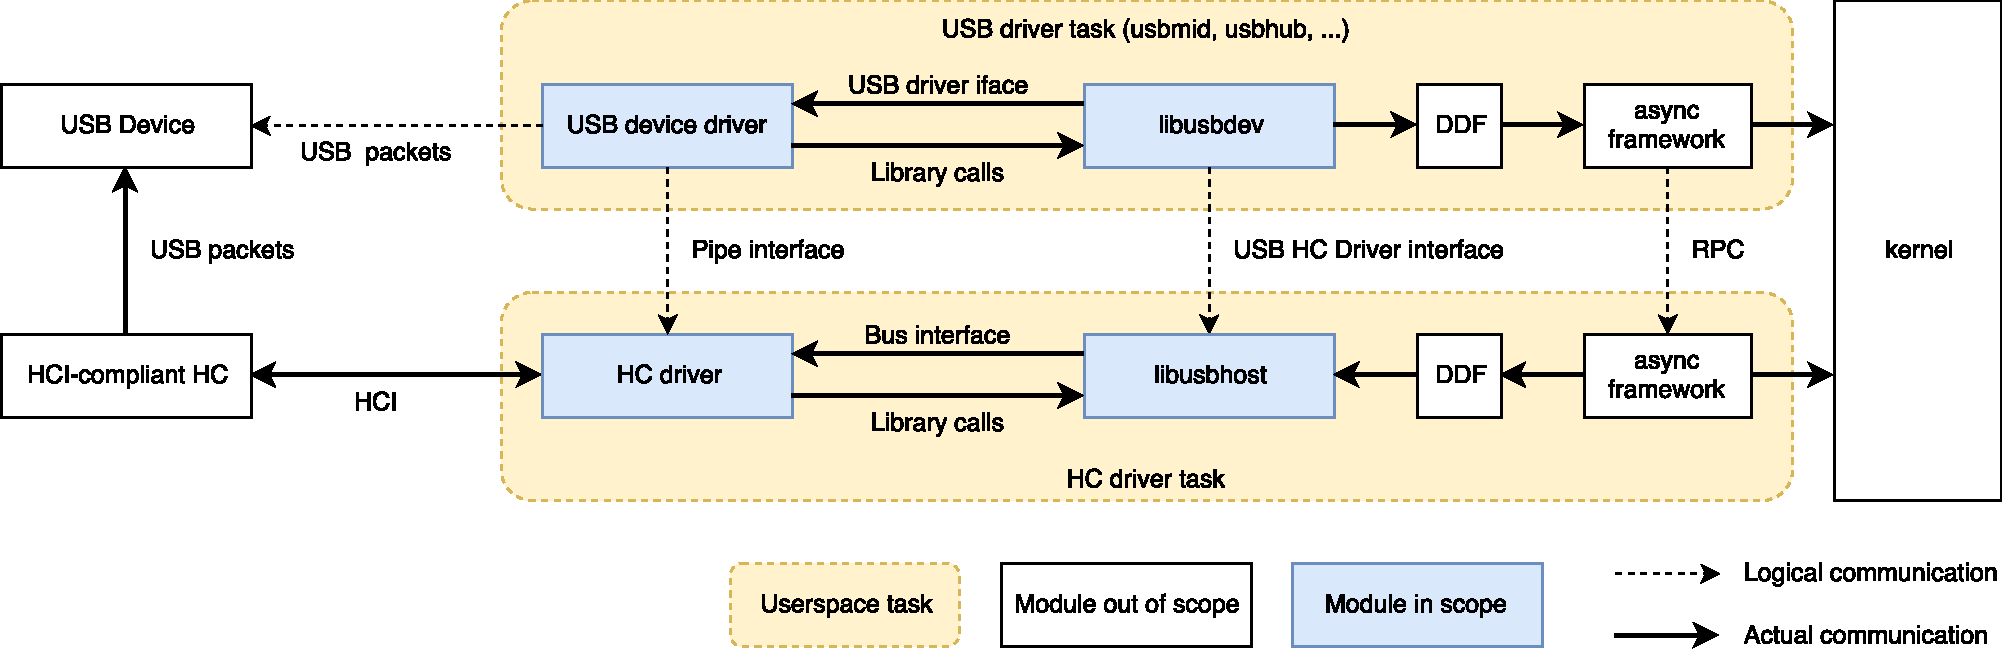
\includegraphics[width=\textwidth]{stack-architecture}
	\caption{The runtime architecture of the USB stack, showing the communication paths}
	\label{fig:stack-architecture}
\end{figure}

At the highest logical level, the USB device driver communicates with the
device using USB packets. The packets are sent through pipes, illusion of which
is created by the \lib{libusbdev} library. The library communicates with the HC
driver using the \texttt{usbhc} driver interface. The drivers actually
communicate using the Device Driver Framework, which in the end uses the
synchronous RPC built upon asynchronous IPC mechanisms in kernel. The
scope of USB stack is limited to the USB device driver tasks, and to the USB
Host Controller driver tasks. Because the USB Device Framework hasn't changed much
in USB 3, our primary focus related to implementing USB 3 support was the HC
driver. The xHCI driver itself was exhaustively explained in the previous
chapter, this chapter explains the modifications needed to implement it.
Furthermore, it contains the modifications needed or supporting the
implementation of other key requirements of the project.

\section{Bus Interface}
\label{sec:bus}

Let us start with the most notable change we introduced to the \lib{libusbhost}
library. Yet before we do, we would like to describe the previous way how
\lib{libusbhost} supported USB HC drivers.

\subsection{Former State}

The library support was mediated by a single structure,
\struct{ddf_hc_driver_t}. This structure contained callbacks implementing
routines to initialize internal structures, start the HC, handle interrupt and
so on. Once the driver's DDF callback \fnc{dev_add} was called, the driver
passed the call to the library along with the \struct{ddf_hc_driver_t}
instance, which described how the HC is to be initialized. In one of the
callbacks, the driver called a function \fnc{hcd_set_implementation}, by which
it configured runtime operations.

From the perspective of data structures, the \lib{libubshost} defined
a structure for an instance of host controller, \struct{hcd_t}, and for
endpoint, \struct{endpoint_t}. Both structures had a field for storing driver
private data. The library also managed a device tree, with the device
structures stored inside DDF function nodes. The device structures were however
private for the library, and apart from two callbacks \fnc{ep_add_hook} and
\fnc{ep_remove_hook} the driver had no information about the devices. Also,
every endpoint could have two callbacks assigned by the driver, which were
called to alter maintenance of the Toggle bit (\fnc{toggle_get/set}).

The main work to be done by the driver is transfer management. For this
purpose, the library defined a structure \struct{usb_transfer_batch_t}, which
was created for every transfer and then passed to the driver's \fnc{schedule}
operation. The batch carried all the information about a USB transfer: target
address, pointer to the data buffer and its size, direction of the transfer and
so on. Along with this data, it carried one of two callbacks (in/out) to be
called after the transfer is finished. This particular callback was set by the
library, depending on the context from which a transfer was scheduled. Transfer
could be initiated either by the HC itself (e.g. reading the device descriptors
to determine match IDs for the DDF), or by the driver of the device via the IPC
interface methods (\fnc{usb_read} or \fnc{usb_write}).

In the first case, the driver called \fnc{hcd_send_batch_sync}, which created
a simple structure with completion flag, and the callback was set to a function
which filled the structure and toggled the completion flag. Then the issuing
fibril polled the completion flag until the transfer was completed. In a case
of a bus transaction issued by the device driver, the callback answered the IPC
call. The asynchronicity of HelenOS IPC fits this scheme perfectly.

Sometimes, if the request modified the internal state of the device (e.g. USB
ResetEndpoint request), the callback was wrapped in another callback, which
reset the endpoint's toggle after completion, and called the original callback.

The overall architecture of using callbacks passed as function arguments and
stored all around was really flexible, but very hard to read and understand.
Instead of simply tracing function calls, we needed to carefully study the
lifetime of the structure to track origins and modifications of these
callbacks.

Also, we felt that keeping driver-private data in a void pointer (with the
burden of maintaining the allocated memory) doesn't fit well for a library of
such a specific purpose. Instead, we decided to start a little revolution here.

\subsection{Current State}

The most notable change we introduced is a clear separation of the callbacks,
forming the interface of the HC driver against the \lib{libusbhost} library,
named the ``Bus interface'' in the figure \ref{fig:stack-architecture}. All the
runtime callbacks the library calls are contained in a single structure,
\struct{bus_ops_t}, which is defined by the driver. It is possible (and
recommended) that the instance of this structure is \mintinline{c}{static
const}, and a pointer to it is shared between all HC's the driver controls. The
names of the callbacks are ``namespaced'' by their first word, to clearly
distinct which entity the operation works with (\fnc{device_enumerate},
\fnc{endpoint_register}, \fnc{batch_schedule}, \dots).

Moreover, we defined a bunch of structures the library shares with the driver.
All of them use pointers and arrays to build a tree of entities the driver
works with. The lifetime of all entities is managed by the library, but the
driver is (with some exceptions) responsible for their allocation and
destruction. That gives the driver great flexibility in where the memory for
the structures will be allocated, and also how large the memory is. None of
them contains a void pointer to store private data, as its not necessary -- the
driver is supposed to allocate memory for a bigger structure if it needs it.

The C standard defines that pointer to a structure is equivalent to a pointer
to its first field. This promise is heavily relied on to implement
``inheritance'' of a C structures. To give an example, suppose that the driver
needs to keep more data about an endpoint. It then creates a structure for it:

\begin{code}
	typedef struct hc_endpoint {
		endpoint_t base;

		bool some_flag;
		unsigned more_data;
	} hc_endpoint_t;
\end{code}

Then, in the \fnc{endpoint_create} bus operation, it is supposed to create the
\struct{endpoint_t} structure. It allocates a space for \struct{hc_endpoint_t}
instead, and returns the pointer to its base field (which we know is the same,
but of different type). Whenever it then receives an \struct{endpoint_t *}
argument to a bus operation, it knows it is safe to typecast the pointer to
\struct{hc_endpoint_t *}, and work with the extended structure containing more
data.

All structures and their relations can be seen on figure
\ref{fig:hcd-memory-structures}. You can see that all of them have pointers to
their parent entities. That allows us to reduce number of arguments passed to
the bus operations, while retaining the flexibility needed to implement the
operations in different drivers. Lets walk through the entities one by one.

\begin{figure}
	\centering
	\label{fig:hcd-memory-structures}
	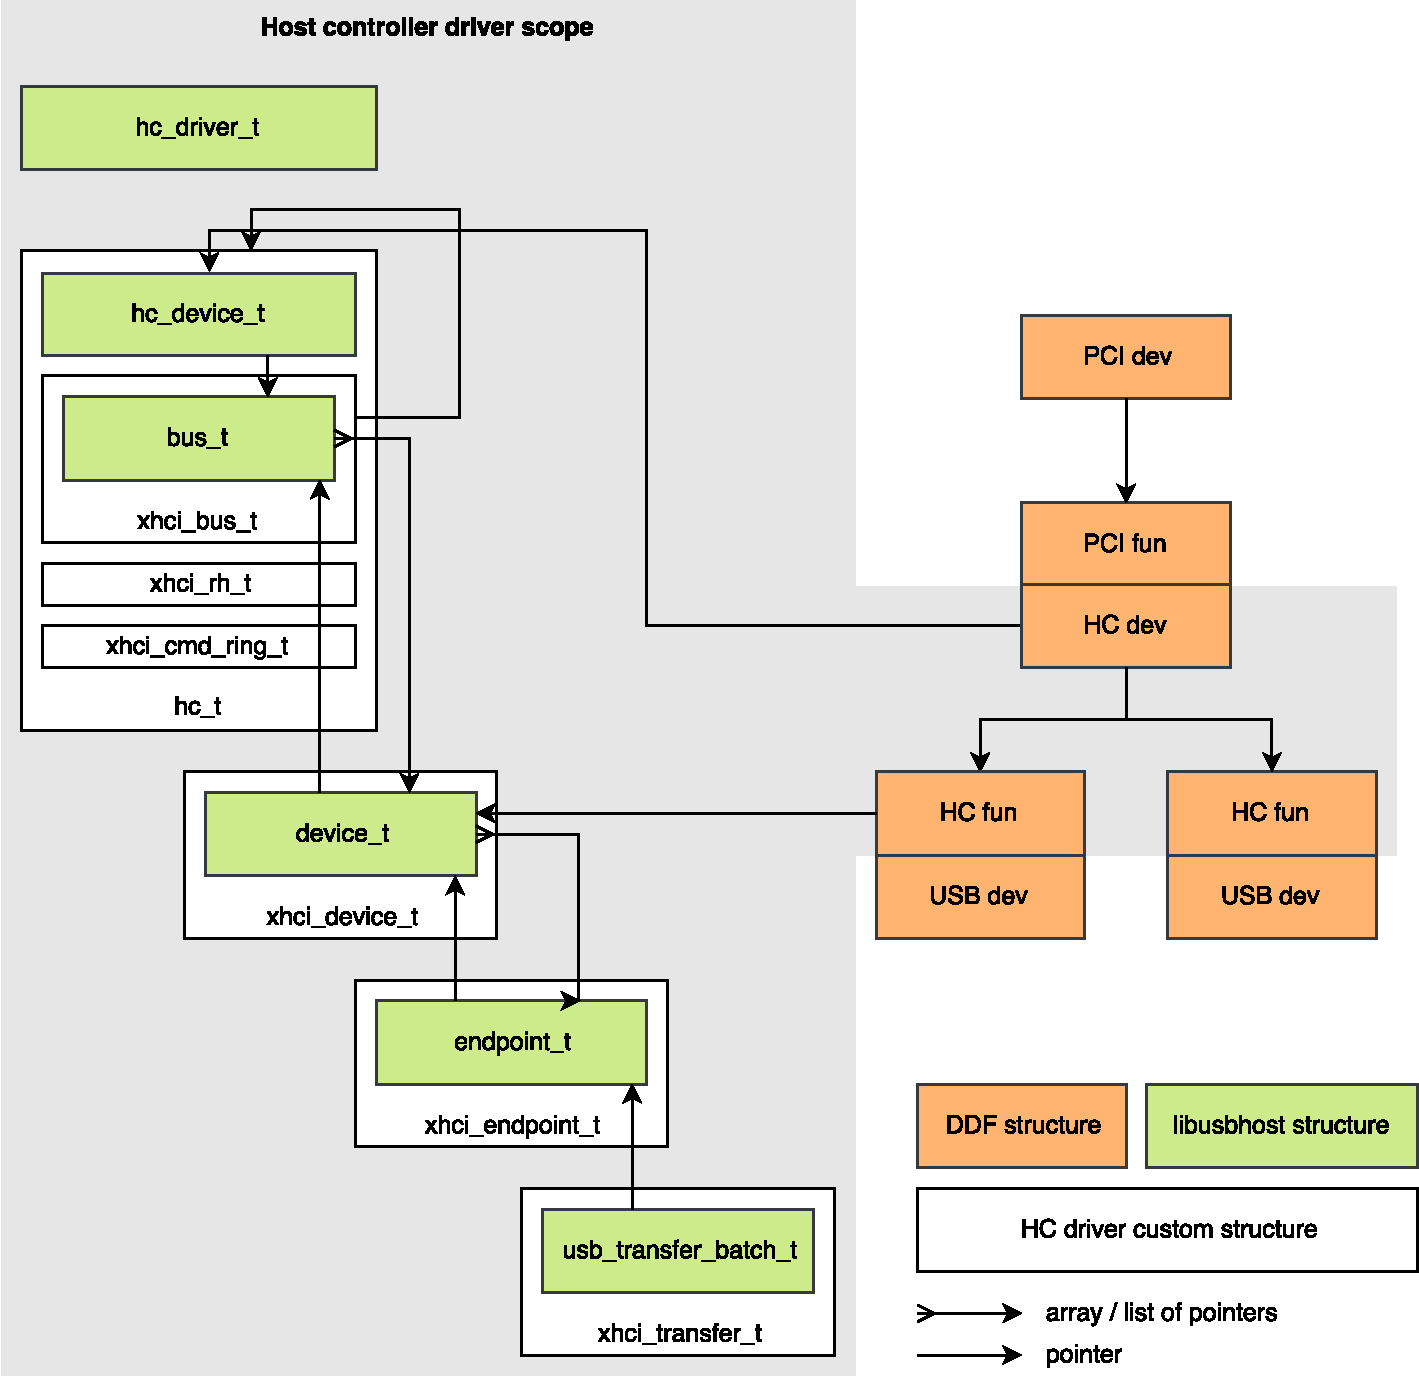
\includegraphics[width=0.5\textwidth]{hcd-memory-structures}
	\caption{Bus structures demonstrated on the example of how xHCI driver uses them.}
\end{figure}

\subsubsection{Structures Shared With the Driver}

\begin{description}
	\item[\struct{hc_driver_t}]
		Represents the driver instance. Created at the task startup (usually as
		a static instance), passed to the \fnc{hc_driver_main}. Contains
		operations to initialize a HC device.
	\item[\struct{hc_device_t}]
		Created by the library for every HC controlled. Contains pointers to
		the DDF device, control function, interrupt-replacement fibril. Shall
		be treated as opaque by the driver.
	\item[\struct{bus_t}]
		Created by the driver for every HC it controls. Manages the reservation
		of default address, keeps the pointer to bus operations. Strictly
		speaking, \struct{hc_device_t} and \struct{bus_t} represent the same
		entity -- the HC instance. They are separated to isolate responsibilities.
	\item[\struct{device_t}]
		Allocated inside the DDF function node for every USB device managed by
		the bus. Contains an array of endpoints registered for that device.
		Also, it contains a list of children \struct{device_t} structures, in
		case this device represents a hub. Because the topology presented to
		the DDF is flattened, this is the only place where the USB tree
		topology is stored.
	\item[\struct{endpoint_t}]
		Created dynamically at the time of registering an endpoint by the
		device driver. Contains information needed for scheduling and
		synchronization of scheduled transfers. Reference counted, as its
		lifetime can extend the lifetime of a device.
	\item[\struct{usb_transfer_batch_t}]
		Created dynamically at the time of initiating a transfer. Ownership
		travels across more entities, more information to be found in section
		\ref{sec:aborting-transfers}.
\end{description}

Now that we know the entities, we can introduce the operations expected to be
implemented by the HC driver.

\subsubsection{Bus Operations}

\begin{description}
	\item[\fnc{interrupt}]
		Process a hardware IRQ. Is passed a bus instance and a 32-bit status
		retrieved from the top half.
	\item[\fnc{status}]
		When the library fails to enable the IRQ, it starts a polling fibril
		instead. The polling fibril calls the status method to retrieve the
		status to be fed to the IRQ handler.

	\item[\fnc{device_enumerate}]
		When a (root)hub finds a new device, the library creates the DDF
		function node, and allocates a \struct{device_t} structure. This
		operation is then called to address the device and create the DDF match
		ids for it.
	\item[\fnc{device_gone}]
		Called when the hub signalizes a device is gone. Not required.
	\item[\fnc{device_offline} and \fnc{device_online}]
		The library calls these when the user requested the device to be brought
		offline/online. More information about this mechanism is in section
		\ref{sec:offline-online}.

	\item[\fnc{endpoint_create}]
		Called when the library needs to materialize an endpoint from the
		endpoint descriptor fetched from the device.
	\item[\fnc{endpoint_register}]
		When the device driver maps an endpoint descriptor, a pipe is created.
		On the HC side, respective endpoint is registered. The registration
		is performed by the library itself, this is just to let the driver do
		the HC-specific work.
	\item[\fnc{endpoint_unregister}]
		When the pipe is closed, the endpoint is unregistered. The HC is
		supposed to terminate all transfers on that endpoint before it returns
		from this operation.
	\item[\fnc{endpoint_destroy}]
		A function to free an endpoint and all allocated information. Called
		once the reference count drops to zero. If not specified, the structure
		is freed by \fnc{free}.

	\item[\fnc{batch_create}]
		Called by the library when a transfer needs to be initiated. If not
		specified, the batch is allocated by \fnc{calloc}.
	\item[\fnc{batch_schedule}]
		Called once the batch is ready to be scheduled.
	\item[\fnc{batch_destroy}]
		Once the batch is finalized and its completion callback is called, this
		function is supposed to free the memory. If not specified, the batch is freed by \fnc{free}.
\end{description}

Some operations do have generic implementation, so that the driver is not
required to implement them, a common behavior is implied. Others are required
only to support a specific functionality -- if not implemented, the
functionality is unavailable. Of course, functionality like the batch
scheduling is optional, but without it the driver is kind of useless.

The only callback that remains separated from the bus is the batch completion
callback. In order to support both synchronous batches from HC itself and
asynchronous batches from IPC, there needs to be a distinction. However, the
callback is no longer abused to implement additional functionality when the
transfer is finished.

To avoid duplicating functionality that was previously in the library and now is
supposed to be implemented by the driver, we created a module
\file{uspace/lib/usbhost/include/usb/host/usb2_bus.h}{<usb/host/usb2\_bus.h>},
which contains an implementation of some
operations relevant for USB2 and below. It implements address allocation, as
only xHC assigns addresses in hardware, older HCs leaves this responsibility on
software. The same holds for bandwidth management, which is further moved to
a separate module \file{/uspace/lib/usbhost/include/usb/host/bandwidth.h}{<usb/host/bandwidth.h>}.

\subsubsection{Development of the Bus Interface Throughout the Project}

At first revisions, the bus interface was a bit richer. Also, it contained more
of the USB2 specifics hardwired -- like the bandwidth management. The impulse
to create the bus interface was the lack of systematic approach in the previous
solution, so it was a bit hard to understand. So we first did a refactoring
process, which moved all callbacks to the bus. For a long time, there was
a kind of runtime virtual binding of functions -- the older HCs used
\struct{usb2_bus_t} as their bus implementation, and overrode some of its
functions. As time passed by, we were able to identify and isolate parts that
could be separated cleanly and reduce the bus interface to its current state.

The result is not that much different from the former state -- only extended by
a few device-related callbacks, as xHC needs to know about devices, former HCs
need not. But the fact we needed to do the refactoring just to understand what
is going on proves the fact this interface must have been cleaned up and
defined more clearly. Also, the sharing of structures reduced the amount of
bookkeeping needed to be done by the drivers. This claim is supported by the
fact that even though we implemented new features and made performance
optimizations, the codebase of former HC drivers shrunk a few kilobytes.

\section{Explicit Device Removal}

One of the project goals is to alter the USB subsystem to allow support for
explicit device removal. Such feature can be found in most modern operating
systems and is often used to ensure that devices are left in a consistent state
after a physical port detachment occurs.

The explicit device removal feature usually provides a frontend interface in
the operating system, through which users can observe currently connected
devices and, if needed, issue a signal to the operating system that their
physical detachment is imminent. Following that, the system is expected to
promptly terminate all ongoing communications with the device and signal the
user back. After receiving the confirmation, user can then safely unplug the
device from the system bus without any risk of interrupting communications,
which could otherwise result in undefined state of the device.


\subsection{Considerations}

In the USB protocol, communications between the host and the device take place
in the form of \textit{transfers}. Depending on its version, the host controller
may have various roles in the realization of these transfers. For that reason,
version-specific modifications are carried out separately in host controller
drivers, whereas common functionality is implemented in the bus module, which is
a part of \lib{libusbhost}.

The disconnection routine for explicit device removal is implemented as follows:
~
\begin{enumerate}
	\item The user signals the intention to disconnect a USB device.
	\item The respective device drivers are notified to end their business (e.
		g. flush buffers or close files), possibly scheduling a multitude of
		transfers to the device.
	\item The HC driver disables the capability to schedule new transfers to the
		device.
	\item The HC driver aborts all leftover active transfers to the device.
	\item The device configuration is dropped, leaving it in the
		\state{Addressed} state, in which it is considered safe to be
		physically removed from the bus.
\end{enumerate}

If the user requests that this routine is rolled back, the steps of the
disconnection routine are just executed in reverse order. The following can
therefore be labeled as a reconnection routine:
~
\begin{enumerate}
	\item The user signals the intention to resume communications with a USB
	device, on which the disconnection routine has been previously performed.
	\item The HC driver configures the device.
	\item The HC driver enables the capability to schedule new transfers to the
	device.
	\item The operating system is notified that the device is reachable and
	matches it to appropriate drivers, which initiate communications with it.
\end{enumerate}

The specialization of both routines is performed in the same way as other bus
module interactions. All HC drivers hand off their DDF and device callbacks to
the bus module, which then calls them back to perform low-level commands related
to specific devices, endpoints and transfers. This way, the high-level logic
contained by the bus module essentially follows the listed descriptions above
and the version-specific extensions are resolved in the respective HC driver
implementations.


\subsection{Offline and Online DDF Signal}

The HelenOS Device Driver Framework includes two user-initiated signals
relevant to the implementation of this feature.

\begin{description}
	\item[Offline Signal]
		This signal informs a driver attached to a DDF node that its managed
		device may be removed in the near future. The driver is expected to
		immediately cease all user operations on the device and unbind its
		child DDF functions, possibly sending a \textit{Device Remove} signal
		to all their attached drivers in the process.

	\item[Online Signal]
		This signal is a logical counterpart to the previous signal.
		It informs a driver attached to a DDF node that its managed device will
		not be removed in the near future. The driver is expected to expose all
		child DDF functions related to the device, possibly sending a
		\textit{Device Add} signal to all their matched drivers in the process.
\end{description}

These signals can be easily issued by the user from the system shell by means
of the \app{devctl} application. See Listing \ref{lst:devctl-offline-online}
for invocation example.

\begin{listing}
	\begin{bdsh}
		# Prepare the unplug high speed device at address 2.
		devctl offline /hw/pci0/00:04.0/usb2-hs

		# We changed our mind. Bring the device back online.
		devctl online /hw/pci0/00:04.0/usb2-hs
	\end{bdsh}
	\caption[Example usage of \app{devctl} to issue offline and online
	signal.]{Example usage of the \app{devctl} application to issue offline and
	online signal to a USB high speed device at address 2. The host controller
	PCI address is \texttt{00:04.0}.}
	\label{lst:devctl-offline-online}
\end{listing}

It follows that these signals can be used for the implementation of the
explicit device removal at the level of USB host controller drivers. For that
reason, \lib{libusbhost} has been extended to handle appropriate DDF callbacks
for functions corresponding to HC's child devices. Their handling is forwarded
to the bus module, which executes the disconnection or the reconnection routine
for the \textit{offline} and \textit{online} signal respectively. In addition,
the transfer scheduling mechanism of the bus module has been extended to permit
scheduling new transfers only to devices, which are in the online state.

The general scheme of stopping communication with a device breaks down to
unregistering all its registered endpoints. The biggest challenge the driver
faces is to abort all currently running transfers on an endpoint that is being
unregistered. The majority of transfers (Bulk, Control, Isochronous,
Interrupt-out) wouldn't pose a problem -- we could just wait the short while
until they are completed, either successfully or not. But then there are
Interrupt-in transfers, which, especially in case of gone device, may not
complete in a timely manner.

\subsection{Aborting active transfers}

It is not possible to ``abort a transfer'' in a generic way, mainly because of
synchronization issues. Before we explain how can a transfer be properly
aborted in various Host Controllers, let us describe the lifecycle of
a transfer batch, a structure representing a transfer in HC drivers.

Currently, USB stack in HelenOS only supports synchronous interface to interact
with pipes. The two methods are called \fnc{dev_read} and \fnc{dev_write}.
Driver calls these methods on pipes, and provides a buffer -- either filled
with data, or to be filled. Once the call crosses the IPC barrier, it is joined
to a call to \fnc{bus_device_send_batch}. This function finds the target
endpoint structure, and passes control to \fnc{endpoint_send_batch}.

There, an instance of \struct{usb_transfer_batch_t} structure is created and
filled with parameters of the transfer. It is then passed to the driver
implementation to be scheduled. The driver typically copies the data to
a buffer suitable for the device, prepares some supporting structures, and
finally, schedules the transfer to the hardware.

Since then, an interrupt may come and finish the transfer in a different
fibril. A transfer is finished by copying the data out from the hardware buffer
to the batch buffer, setting the error code and calling a completion callback.
This callbacks answers the original incoming IPC call, causing the \fnc{dev_read/write}
function to return. After that, the transfer batch is destroyed.

But that's not the only scenario that may happen. From the moment a transfer is
created, a pointer to it must not be forgotten, otherwise the caller would
never return. But on the other side, once the pointer to batch is stored
somewhere, the transfer might be aborted at any time. Furthermore, once the
transfer is scheduled to the hardware, the buffers must not be deallocated
until the driver is sure that the hardware won't use them anymore.

This synchronization problem might be resolved by locking the batch and
reference counting, but then different problems would arise (e.g. a transfer
could be finished after the endpoint was successfully unregistered, just
because we cannot know if there's any). So, we decided to take a different
approach.

As the interface is synchronous (and it doesn't make much sense to make it
asynchronous, unless under special conditions), and the endpoint is assumed to
be available for one driver only, there's no point in having more than one
transfer active at a time. So, we store the pointer to a batch inside the
endpoint structure, in the field \struct{active_batch}. This field shall not be
accessed, unless the endpoint guard is locked.

The driver shall modify this field only by calling two methods, which ensure
the proper semantics: \fnc{endpoint_activate_locked} and \fnc{endpoint_deactivate_locked}.
Both of them are to be called with the guard locked. An endpoint is said to be
\emph{active}, if there's an active transfer scheduled. Once the endpoint is
activated and the guard released, the batch must be assumed to be already
finished or aborted. In the counterpart process, when the driver wants to
finish or abort transfer, it needs to obtain the endpoint guard, check if the
transfer is still the active transfer, and then deactivate the endpoint.

In other words, the ownership of the batch is transferred from the calling
fibril to the endpoint once activated, and to the finishing/aborting fibril by
deactivating the endpoint. Only the owner of the batch is allowed to finish it.

Following this scheme a driver can be sure a batch is always finished once and
only once. But in our thoughts, we haven't yet covered that the buffers of the
batch are owned by the Host Controller while the batch is scheduled. Because of
that, drivers need to implement aborting transfers themselves.

The version-specific part of the implementation is discussed in the next sections.


\subsection{UHCI, OHCI and EHCI specifics}

All three HCI's that were supported prior to our project have similar
structure with regard to what is required to implement transfer aborting. Let us
first describe very briefly how these controllers handle transfers.

Generally, all three host controllers require driver to create a system of
linked structures in memory (for UHCI and OHCI, restricted to the lower 4 GBs
of addressable space). The names and guts differ, the structures however
describe a linked chain of queues. Queues are then filled by transfer
descriptors, which describe USB transfers to be done. Once the transfer is
done, its descriptor is flagged, removed from the queue and if the descriptor
is marked, the host is interrupted. More specific information can be found
either in respective specifications, or in the documentation of the HelUSB
project.

At the time of receiving an interrupt, the host does not know which transfer
was finished, so it has to check all pending transfer descriptors for the
completion flag. In case all the transfer descriptors of a transfer are
completed, the driver may finish the transfer.

When aborting a transfer, the driver must make sure the controller is not using
any of the allocated buffers. It is allowed to modify the queues while the
controller is scanning them, the modifications must however follow an order in
which the consistency of the structure is guaranteed at any time. After it
does, it must notify the driver that the structure has changed, in order to
force the controller to clear its caches (EHCI only).

Because the driver is polling the transfers for completion, the first thing
we (as a driver) have to do to abort a transfer is to remove it from the list
of pending transfers. As the list modification is synchronized, we can be sure
no other fibril will ever complete the transfer. After that, we can finish it
ourselves with an error. Note that in this case it is unknown to driver whether
the transfer was completed or not -- but since the driver is unregistering an
endpoint, the device must already be in a state in which it expects removal.

The removal itself is not that easy as one would expect, because it involves
two locks. While scheduling the transfer, we (potentially) need to wait, until
the endpoint is free to be activated, so we need to take the endpoint lock first.
On the other hand, when scanning the pending list, we cannot know the
endpoints, and therefore cannot lock them in advance. The resolution of this
conflict is different in every driver

% TODO: In UHCI, it is currently broken, and it struck me while writing the
% documentation. Too late for me to fix it now, gotta go sleep.

In OHCI and EHCI, transfers have to be prepared with previous transfers in
mind. To avoid the conflict, we changed the list of pending transfers to list
of pending endpoints. The endpoint's reference in this list is counted, and it
is possible to check whether the endpoint takes part in the list. We can remove
it if it is without holding the endpoint lock, and then finish the transfer
without holding the list lock, thus avoiding the ABBA deadlock completely.

From the further perspective, these controllers do not have an internal state
for individual devices and endpoints, so the deconfiguration and its rollback
is an operation on software-state only. As such it is already done completely
by the \lib{libusbhost} library.

\subsection{xHCI Specifics}

Since xHCI is the latest HC interface implementation, a lot more is done by the
hardware for the HC driver in comparison with previous versions. The concept of
xHCI command ring leads to very elegant implementation of the required
functionality on the HC driver part.

For the purpose of aborting active transfers, the xHCI features an explicit
\textit{Stop Endpoint} command, which instructs the HC to abort all transfers
to a specific device endpoint. This command is issued by the HC driver for all
removed device endpoints, which are active at the moment of the request.
Furthermore, device configuration is dropped along with all remaining endpoints
by issuing a \textit{Configure Endpoint} command with the DC (deconfigure)
flag.

Reconnection is quite straightforward and requires only that the HC driver
issues a regular \textit{Configure Endpoint} command in order to transition the
device from the \state{Addressed} state back to the \state{Configured} state.


\subsection{Driver Support}

Since the existing USB drivers were quite incomplete, their implementation has
been extended to add support for explicit device removal. This mostly lead to
novel approaches to deallocation of device-related memory structures, which is
often performed in the \fnc{device_remove()} and \fnc{device_gone()} driver
callbacks.

For instance, a number of drivers required that an implementation of
\fnc{device_remove()} is created in the first place. Quite so often, the
existing implementation of \fnc{device_gone()} has provided a good starting
point, given that both functions have to deal with USB device's demise. The
fundamental difference was that while \fnc{device_gone()} merely dealt with
the fallout of unexpectedly unplugged device, \fnc{device_remove()} had the
opportunity to tie up all lose ends prior to the physical detachment of the
device.

This posed a problem, especially in HID and hub drivers, which heavily relied on
polling of interrupt endpoints. Since polling was a synchronous operation from
the device driver's point of view, a polling fibril has been created when the
driver started managing the device. When the device was unplugged, the polling
operation failed with error, waking up and effectively terminating the fibril in
the process. Since no explicit joining mechanism was available, the
implementation of \fnc{device_gone()} merely spinned a limited number of times,
waiting for the polling fibril to die. This mechanism was however unsuitable for
\fnc{device_remove()}, since the fibril would not awaken due to an error caused
by the physical disconnect, which has not happened yet.

This lead to complete refactoring and extension of the USB device polling
mechanism, which is described in detail in Section \ref{polling-refactoring}.
In summation, the new version of the mechanism allows device drivers to join
their polling fibrils and consistently wake them up in order to avoid deadlocks.

To actually stop the polling in the \fnc{device_remove()} callback, the device
driver has to trigger a transfer abort inside the HC. There's no sensible way
of how to allow a driver abort its own transfer, which wouldn't introduce
potential memory leaks inside HC or synchronization problems. So we decided
that the driver will have to unregister the endpoint as the only way to abort
a currently running transfer (and also disable scheduling of new ones). The
device's endpoints (or, at this layer already called pipes) are completely
managed by the \lib{libusbdev} library. Previously, their lifetime was strictly
tied to the lifetime of the handled device. There are only two possible
ordering of these two operations:

\begin{enumerate}
	\item Close the pipes after the \fnc{device_remove()} callback returns.
		After that, the polling fibrils will end and destroy their structures.
		The library USB device structure will have to be reference-counted and
		the counter will be managed by the driver to account for polling
		fibrils.

	\item Close the pipes prior to calling \fnc{device_remove()}, effectively
		destroying the only reason why this callback exists, and make the
		expected removal equivalent to the unexpected one.
\end{enumerate}

\noindent It is pretty obvious that we had to choose a completely different approach. So
we came up with three more options:

\begin{enumerate}
\setcounter{enumi}{2}
	\item Introduce a new callback, e.g. \fnc{device_removed()}, to be called
		after the pipes are closed. The removal would be split into two phases:
		first, in \fnc{device_remove()} the loose ends are closed and the
		device is brought to a state expecting removal, then in
		\fnc{device_removed()}, the polling fibrils are joined and structures
		are destroyed.

	\item After calling \fnc{device_remove()} and closing the pipes, call
		\fnc{device_gone()}.

	\item Allow the driver to close individual pipes imperatively.
\end{enumerate}

At first, we decided to go with option 3). But it was yet another callback, we
didn't come up with a name that wasn't so similar and yet was clear, and
finally, the \fnc{device_removed()} callback implementations were very similar
to \fnc{device_gone()}.

The option 4) seems reasonable at the first look, but it would create
inconsistency between DDF drivers and USB drivers, which would be very
confusing for developers. \footnote{Actually, some team members think this
behavior shall be present in DDF too, but we didn't open a discussion with
HelenOS developers.}

In the end, the only option left was letting the driver close its own pipes. So
we introduced a new library call \fnc{usb_device_unmap_ep()}, which does
exactly that. The new library polling mechanism closes its pipe automatically,
but this functionality is usable in any driver for any endpoint.

The implementation of explicit device removal support for the rest of the
drivers was a trivial extension of their previous functionality.


\section{Polling Mechanism Improvements}~\label{polling-refactoring}

As hinted by the previous section, the USB device endpoint polling mechanism has
been completely refactored.


\subsection{Before State}

In the original state, USB device drivers had to configure polling using a
configuration structure \struct{usb_device_auto_polling_t}, then pass this
structure to one of four functions:

\begin{itemize}
	\item \fnc{usb_device_auto_poll()},
	\item \fnc{usb_device_auto_poll_desc()},
	\item \fnc{usb_device_auto_polling()},
	\item \fnc{usb_device_auto_polling_desc()}.
\end{itemize}

These functions copied the configuration and started an automated polling
fibril, which interacted with the deice driver using callbacks specified in the
configuration structure. At the end of the polling, the fibril deallocated all
of the resources and terminated.


\subsection{Motivation}

There was a number of problems with the status quo:

\begin{itemize}
	\item The semantics of functions used to initiate polling was not clearly
		distinguished by their name (and neither their documentation).
	\item In addition, the polling functions had a high number of arguments,
		which opened possible room to device driver errors due to their
		misinterpretation (or further API changes in the future).
	\item The polling fibril was detached at the moment of polling start and
		could outlive the device in the driver's memory, then fail later when
		accessing memory, which was already freed in \fnc{device_remove()} or
		\fnc{device_gone()}. Some drivers bypassed this by spinning in these callbacks,
		waiting for the fibril to terminate. However, if the fibril was still
		polling even after a number of attempts, a non-zero error code was returned,
		rendering the entire DDF function (along with its subtree) in a defunct
		state.
	\item The driver was unable to inspect the state of the polling fibril
		directly, so often a flag had to be created and maintained by polling
		callbacks.
	\item A distinct subset of polling parameters were not configurable and were
		hard-assigned their default values inside function implementation. If the
		driver wanted to change any (and not necessarily all) of such parameters, it
		had to specify all the values by itself. Because the constants were
		hard-coded in the implementation, the driver then usually had to copy the
		values.
\end{itemize}


\subsection{Modifications}

\begin{figure}
	\centering
	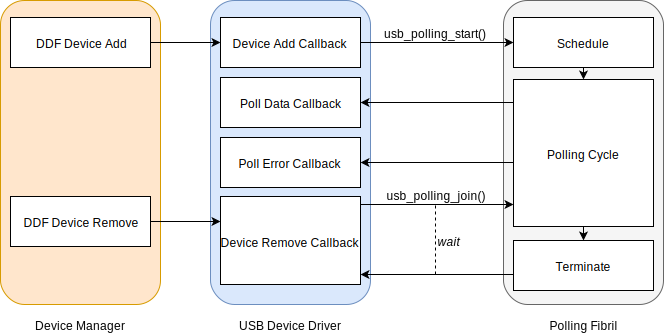
\includegraphics[width=0.8\textwidth]{usb-polling}
	\caption[USB device polling interactions diagram.]{A diagram of interactions
	between the Device Manager, USB device driver and one of its polling fibrils
	during its lifecycle.}
	\label{fig:usb-polling}
\end{figure}

The configuration structure \struct{usb_device_auto_polling_t} has been renamed
for simplicity sake to \struct{usb_polling_t}. Instead of serving as a one-time
configuration structure during polling initiation, its role changed to represent
the entire instance of the polling process throughout its lifetime.

Introducing standard functions such as \fnc{usb_polling_init()} and
\fnc{usb_polling_fini()}, the device driver is now fully responsible for the
ownership of the structure. This is convenient, since drivers often have their
own structures for device data, where \struct{usb_polling_t} can be placed as a
field, dropping the need for additional calls to \fnc{malloc()} and
\fnc{free()}. In addition, this resolves the problem with default values of
various configuration parameters, since in \fnc{usb_polling_init()} all
parameters are assigned their default values and device driver can override only
those desired.

All four of the original polling initialization functions were unified into a
single function \fnc{usb_polling_start()}. Since there is now a clear structure,
which represents the polling instance, the arguments of the original four
functions were moved to \struct{usb_polling_t}, where they are clearly named and
documented, preventing any possible errors from their misinterpretation. Suffice
it to say, that the original four functions mostly fulfilled the role of syntax
sugar, which is now rendered unnecessary, given the fact that default values of
configuration parameters are pre-filled in the polling structure.

Lastly, the API was extended with the \fnc{usb_polling_join()} function, which
closes the polling pipe and consistently waits until the polling fibril
terminates. This function addresses the problem of spinning in driver's
\fnc{device_remove()} or \fnc{device_gone()} callbacks, or possible negligence,
which may result in the polling fibril outliving the device and then accessing
invalid memory. Calling this function in this context will result in the
immediate and synchronous termination of the polling mechanism prior to
deallocation (as depicted in Figure \ref{fig:usb-polling}).

Furthermore, the exposure of internal polling parameters now gives device
drivers more creativity in their approach to polling. For instance, drivers can
now inquire about the state of the polling fibril without the need to have a
private flag maintained by their polling callbacks. The drivers can also change
polling parameters such as request size or polling delay mid-flight, which is a
more flexible approach than to stop polling, change parameters and then start
polling again (note that stopping polling at will was not supported by the
previous implementation without generating actual errors from the hardware
device).

A nice minimalist example of the new polling mechanism usage can be found in
Listing \ref{lst:polling-example}

\begin{listing}
	\begin{code}
		static usb_polling_t polling;
		static uint8_t buffer[13];

		static bool callback(usb_device_t *dev, uint8_t *buffer, size_t size, void *arg)
		{
			printf("Have data!/n");

			// Return true if we wish to continue polling.
			return true;
		}

		static void demo()
		{
			// Initialize.
			usb_polling_init(&polling);

			// Configure.
			polling.device = /* some usb_device_t here */;
			polling.ep_mapping = /* some interrupt(in) endpoint of the device */;
			polling.buffer = buffer;
			polling.request_size = sizeof(buffer);
			polling.on_data = callback;

			// Start polling.
			usb_polling_start(&polling);

			// Sleep synchronously for a while.
			async_usleep(10000);

			// End polling and clean up.
			usb_polling_join(&polling);
			usb_polling_fini(&polling);
		}
	\end{code}
	\caption{Minimal usage example of the new USB device polling mechanism.}
	\label{lst:polling-example}
\end{listing}



\section{A Library Module for USB Hubs}
\label{hub-port-refactoring}

We introduced a new module to support writing hub drivers:
\file{uspace/lib/usb/include/usb/port.h}{usb/port.h}. It solves the problem of
hub drivers that events are announced through a single channel, even though
they need to wait for each other. The implementation of this module was
motivated not only by the need of refactoring, nor because we wanted to share
the functionality with the xHCI driver, but because the previous implementation
of \lib{usbhub} driver synchronized the fibrils wrong. There might have been
situations in which two fibrils were spawned and enumerated the same device.

To solve the issue a state information is managed for every port, represented
by the structure \struct{usb_port_t}. It contains the current port state, one
of the following:

\begin{description}
\begingroup \leftskip=1cm \rightskip=\leftskip
\setcounter{enumi}{-1}
	\item[\state{Disabled}]
		There has been no activity on the port yet, or it is already over.
		Initial state.

	\item[\state{Connecting}]
		A connected event came, the enumerating fibril was started. It hasn't
		finished yet, so the device is not enumerated yet. Also, the device is
		still connected, no error event came while the connecting is in
		progress.

	\item[\state{Enumerated}]
		The device was successfully enumerated, so it has to be removed after
		it will be disconnected.

	\item[\state{Disconnecting}]
		A disconnected event came after the device was enumerated, so
		a removing fibril was started.

	\item[\state{Error}]
		An event about the device disconnection state came while the
		enumeration was in progress, so the enumeration fibril has to be
		stopped. This is achieved by returning \macro{EINTR} from the blocking
		functions.

\endgroup
\end{description}

The basic synchronization invariant is that the state never changes unless the
guard is locked. It is expected that the guard is not held for a long time, so
the fibril generating events shall not be blocked indefinitely. The only
exception being the final phase of enumeration (announcing the device to the
bus), which once started, cannot be easily interrupted -- but this operation on
the bus is also expected to run for a limited time only.

The scheme of states and allowed transitions can be seen on figure
\ref{fig:port-states}.

\begin{figure}[h]
	\centering
	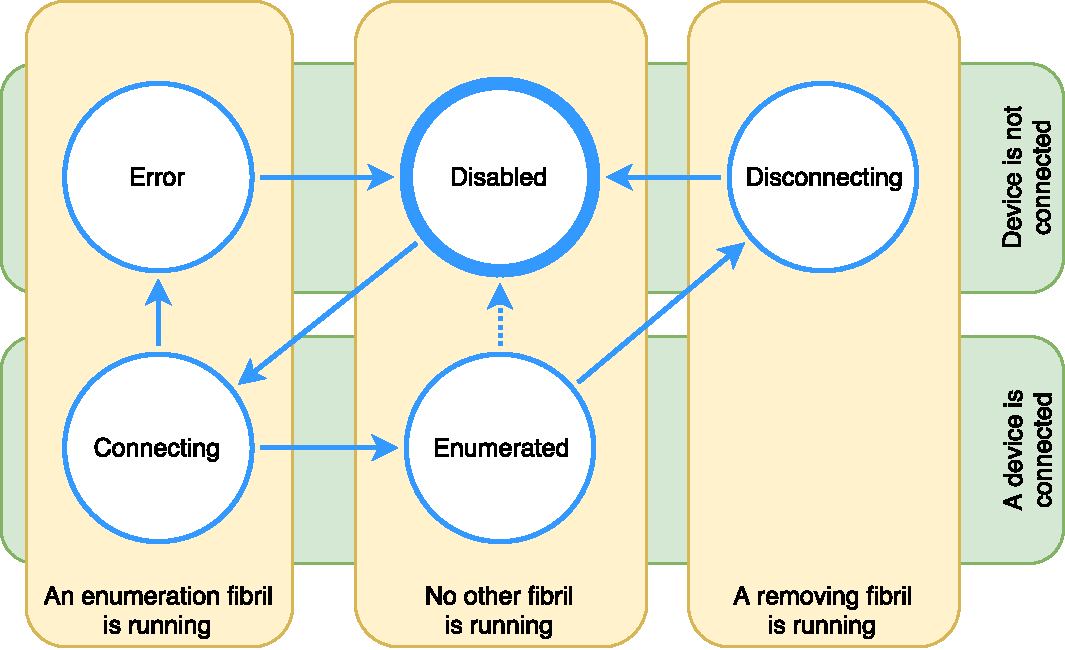
\includegraphics[width=0.6\textwidth]{port-states}
	\caption{A graph of port states and their transitions.}
	\label{fig:port-states}
\end{figure}

The transitions are triggered by delivering events to the module. This is done
by calling following functions:

\begin{itemize}
	\item \fnc{usb_port_connected}
	\item \fnc{usb_port_disabled}
	\item \fnc{usb_port_enabled}
\end{itemize}

The \fnc{connected} and \fnc{disabled} functions take a callback as an
argument. If the respective state transition is triggered, this callback is run
in a separate fibril. These functions can block to obtain the port guard, and
the \fnc{disabled} event can furthermore block while waiting for the
enumeration fibril to terminate. But before it does, it makes sure the worker
will be notified as soon as possible.

To make it work, the callbacks must not block while holding the guard. They
can, however, wait for the enabled event, signalling the completion of port
reset, using a function \fnc{usb_port_wait_for_enabled}. The caller is required
to check the return value of it -- it can either finish with \macro{EOK},
timeout with \macro{ETIMEOUT} or be interrupted with \macro{EINTR}. The enabled
event is sent by calling the function \fnc{usb_port_enabled}.

When this fibril management is separated, an implementation of USB hub driver or
root hub driver is very simple. The hub driver just initializes the
\struct{usb_port_t} structure for every port it manages, then waits for events
from the hardware (either by poling the \textit{Status Change Endpoint}, or by
waiting for an interrupt), and forwards the events to this module, providing an
implementation of the enumeration and removal process.

One last thing to note is what to do when the structure is finalized, but
a device is still connected. It might happen that there is a subtree of devices
and hubs being removed because the subtree root $R$ has been unexpectedly
removed. In that case, a port disconnect is delivered to the parenting hub,
which triggers the device removal process. The hub $R$ then receives the DDF
signal \fnc{device_offline}, and starts removal of its own children. But
there's a catch: USB hierarchy is presented as a flat one to the DDF framework.
That means that the devman has no clue about hubs (it sees them as ordinary USB
devices), and considers that all of them are connected to the HC directly.
Device removal is prepared for the situation that device will remove also its
\textit{children} devices, but serializes removal of \textit{sibling} devices.
Therefore, recursive removal of hubs creates a deadlock in devman.

Fortunately, the HC driver must be prepared for badly written drivers, so it
cleans up after the device function is unbound. This cleanup includes also
removal of its former children devices -- so the workaround for this problem is
simply leaving those devices connected, as the HC will remove them itself. This
state transition is denoted by dotted line in the graph, and is triggered by
finalizing the port structure while a device is enumerated.

\section{USB Tablet Driver}
\label{sec:usb-tablet-driver}

This modification is very standalone and seemingly simple, yet very useful and
appreciated. We extended the HID driver to support absolutely positioned
devices. That means, one can now connect a USB tablet and it will work in
HelenOS. If you are still wondering what this could be useful for (people using
USB tablets are usually graphic designers or photographers, not microkernel
developers), try running QEMU with an emulated one:

\begin{bdsh}
$ qemu-system-x86_64 -enable-kvm -usb -device usb-tablet -boot d -cdrom image.iso
\end{bdsh}

When using mouse with relative positioning (PS/2, USB mouse), one has to first
click inside the window of QEMU to let it grab input. To release it again,
a special key combination (for current QEMU Ctrl+Alt+G) must be pressed. When
using an emulated USB tablet instead, the mouse is not ``locked'' inside the
window, but it can freely move in and out and still be registered by the guest
OS.

\section{DMA buffers}
\label{sec:dma_bufs}

A simple but repeated scenario gave rise to another new submodule of
\lib{libusbhost}. It started as a thin abstraction, and its purpose grew to
a major performance optimization targeting the whole system. Therefore, we plan
to discuss with HelenOS core developers to incorporate it in other drivers as
well.

\subsection{The original purpose}

A common task for drivers is allocating memory for buffers, that are accessible
for DMA. Often there are some restrictions given by the hardware driven -- the
buffer must be placed in the lower 32bit addressable space, it has to be
aligned, physically contiguous, or possibly not crossing a page boundary.

Even if the buffer is intended for the hardware use only (like xHCI
scratchpads), the driver must keep the pointer to where the buffer is mapped
inside its virtual address space in order to release the memory once it is not
needed anymore. Hardware devices do not share the virtual address space with
the task though, so the driver must always obtain also the physical address of
the buffer. To satisfy all of these requirements, the HelenOS kernel offers
a specialized API. The driver just needs to call a function
\fnc{dma_map_anonymous}, and is given both the virtual and physical address. It
is able to specify its requirements using flags. This API is powerful, but
complex and inconvenient to use.

The authors of the former USB stack addressed the complexity by creating
utility functions in
\file{uspace/lib/usbhost/include/usb/host/utils/malloc32.h}{<usb/host/utils/malloc32.h>}.
These functions offer
a familiar interface of \fnc{malloc}/\fnc{free}. The \fnc{malloc32} function
intentionally discards the physical address provided by
\fnc{dma_map_anonymous}, in order to be simple to use. To retrieve the physical
address later, one can use another utility function, \fnc{addr_to_phys}. This
one is a simple wrapper for a syscall.

Even previous authors of the USB subsystem were aware of it being a syscall,
and tried to cache the physical address where it would be used unnecessarily
multiple times. The usage scheme of these functions then grew wild: the memory
was allocated by \fnc{malloc32}, just to be translated by \fnc{addr_to_phys} on
the next line. These two pointers were then stored inside the same structure.

Being aware of this use-case, we created a different submodule for allocation
of DMA buffers. Instead of a plain pointer, the caller uses a structure called
\struct{dma_buffer_t}. When the buffer is no longer needed, it is freed by
calling \fnc{dma_buffer_free}. As the translation to physical address is
usually needed in a sequential manner shortly after allocation, we cache the
physical address of the base of a contiguous chunk and compute the resulting
physical address ourselves. Therefore, \fnc{dma_buffer_phys} might be used to
efficiently translate a virtual pointer to a physical one.

When the buffer is contiguous in memory, it's easy to calculate the physical
address ourselves, without a help of the kernel. To obtain a physical address
for a concrete position in the buffer, one just needs to call
\fnc{dma_buffer_phys}, which translates a virtual address pointing inside
a buffer to a corresponding physical address.

One more reason to drop the previous \fnc{malloc32} helpers completely is that
developers that are beginners to HelenOS might see \fnc{malloc32} as a weird
name for an ordinary \fnc{malloc}, and start using it to allocate ordinary
memory, which is very wasteful and expensive.

Even authors of the previous implementation started to overlook fact, that
\fnc{malloc32} actually allocates a whole page, and implemented some operations
very prodigally. The most notable occurrence was in transfer handling -- every
transfer descriptor and queue head was allocated in a separate memory page.
From the performance point of view, allocation and clearing of several memory
pages just to issue one short transfer is an extreme overhead. Furthermore,
a TD can describe at most 8KB transfer, so a linear number of TDs are used.
On the other hand, it is also waste of memory to allocate the memory in
advance. So we at least merged all the needed structures to one allocated
buffer to reduce the overhead to one page only.


\subsection{Policies}

To accomplish a goal described in the following chapter, we needed a way how to
express constraints put on DMA buffers by individual drivers. After evaluating
the individual needs, it came out that there are just two of them:
a requirement of using 32-bit addresses, and a requirement of physical
contiguity. However, the contiguity is not just binary (either fully contiguous
or not). For example, xHCI-compatible controller is able to do bytewise
scatter-gather. That means it can handle also non-contiguous buffers,
translated as a scatter-gather on pages. On the other hand, every TRB can
describe a 64KB block, so it can benefit from the buffer being contiguous by
using less TRBs per transfer.

We used our benchmarking system to measure performance of issuing transfers.
The scenario contains a QEMU virtual device (tmon) receiving our data and
a software driver of this device issuing transfer. The most important aspect of
the testing is that neither of these two entities actually care about the data
being transmitted -- the driver just allocates a buffer of garbage and sends
it. The receiving side just counts the size of the received data. It is
a completely artificial scenario, but allows us to measure the overhead induced
by handling transfers, thus limiting the possible performance in real scenarios.

We measured the maximum performance of bulk transfers of a 64KB buffer. That is
the maximum size of data transferred over IPC in HelenOS. When we relied on the
buffer being contiguous, we could always issue single TRB per transfer. When
not, we had to split the transfer to 16 TRBs. In the first case, the average
performance was around 300~MB/s, in the second one, it dropped to 60~MB/s. That
shows that the overhead is significant and we should use as large TRBs as
possible.

It seems that the best solution would be to allocate chunks of 16 pages and
split the data accordingly. However, using a buffer vector would introduce yet
another API which would drivers have to use instead of a standard one. And with
the experience with IO vectors from QEMU, we decided this is not a good option.
The more when the same task can be solved by a slightly smarter kernel
allocator, mapping the chunks into contiguous virtual memory. But anyway, we
needed a way to express how big the chunks have to be.

Let us introduce another scenario, which could've worked if we had the power.
Imagine a VFS server trying to copy 16 megabytes of data from hard drive to
a flash drive. Let's say that the hard drive driver is capable of arbitrary
scatter-gather operations, but handles 32-bit addresses only. On the other
side, there is an xHC, which can handle 64-bit addresses, but it works best
with 64KB-contiguous chunks. However, in between there sits a USB mass storage
driver, which (just to demonstrate the idea) can issue only 32KB transfers,
so it splits bigger ones to multiple calls. In an ideal world, the VFS driver
would allocate a 16~MB buffer that is in the lower 4 gigabytes of memory, and
every 32KB chunk of it is physically contiguous. Then it would share the buffer
using IPC memory sharing capabilities, so that the hard drive driver loads the
data in it. Then, without any copying, the VFS server would share the buffer
all the way down to the xHCI driver, which would issue 32 KB transfers as
ordered by the mass storage driver with the data directly, again without any
further copying.

This level of copy-free efficiency is thought to be reasonably possible only in
unikernel systems. But for an unknown reason we were too enthusiastic to let
it be and decided to do a little experiment, designing a system which would
allow this scenario to happen even in HelenOS.

The answer to all these issues is surprisingly simple. We use a pointer-sized
bitmap called \struct{dma_policy_t} to carry flags. The flag on bit $i$ denotes
that the buffer may be split into $2^{i+1}$B-sized chunks that are physically
contiguous. As the minimal granularity is \macro{PAGE_SIZE}, the lower bits can
be used to carry different flags. Currently, we use just one to denote the
32-bit restriction.

The policy is a part of the pipe description, which is passed from HC driver to
the USB device driver. It may than allocate a buffer according to this
policy, and be sure that the HC driver will be able to use it directly. The
policy a buffer is allocated with is passed along, for the HC driver to check.
Because we generally trust the driver, there is no further checking. We do not
trust the human writing it though so the policy is not automatically assumed
but must be passed explicitly with the buffer pointer. This has another benefit
-- in case the policy is not exactly satisfied (e.g. the xHCI driver is given
a non-contiguous buffer), it may decide that instead of bouncing it, which is
expensive, it just uses a page-sized chunks for scatter-gather.

If this mechanism would be adopted by the rest of the system, the scenario
described above would start with the VFS driver fetching policies from the
lower-layer drivers. The HC driver would respond with a policy requiring 64KB
chunks, but it would be modified by the mass storage driver to loosen the
contiguity requirements, because it knows that the limit is actually 32KB. This
can be done by a simple bitwise AND operation. From the other side, the hard
drive driver would respond with a policy requiring 32-bit addresses. The VFS
driver then computes a bitwise OR, creating a policy that satisfies both sides.

\section{Memory Sharing}

As promised in the previous section, we modified the interface of host
controller driver. Instead of sending large data through IPC, which requires
kernel to copy data from one task to another, we now use IPC memory sharing.
While it might be actually slower for small transfers (latency benchmarks shows
the difference is not relevant), it makes a big difference for large transfers.
Utilizing the DMA policies described in the previous section, we achieved
a copy-free path from USB device driver to the xHC.

By switching to memory sharing, we released the size limit of one transfer --
the shared memory area might be arbitrarily large, as opposed to the 64KB
artificial limit imposed by the kernel on data transfers. That introduced the
need to actually split transfers to multiple TRBs if needed, so the benchmarked
performance of previously described scenario dropped to 200~MB/s. However, by
using transfers of size 16~MB, we can reach a measured bandwidth of around 1.3~GB/s.
As the theoretical limit of the USB~3.1 (gen.~1) bus is 671~MB/s, we can say that the
bottleneck is no longer in the xHCI driver.

As for the other drivers, the benchmarks on EHCI shown an improvement at 64KB
blocks from 20~MB/s to 25~MB/s, but by using much bigger blocks (larger than 32
MB) we were able to reach 360~MB/s. Again, this is much bigger than the
theoretical limit of 60~MB/s for the bus due to the test nature and virtual
environment.
